% This is samplepaper.tex, a sample chapter demonstrating the
% LLNCS macro package for Springer Computer Science proceedings;
% Version 2.20 of 2017/10/04
%
\documentclass[runningheads]{llncs}
%
\usepackage{graphicx}
\usepackage[section]{placeins}

\begin{document}
%
\title{Intelligent Energy Management}

\author{Group Name: Sandesh Kenjana Ashok \and
Kartik Nayak \and
Mirac Coskuner}

\institute{Service Computing Department, IAAS, University of Stuttgart
\email{kartik.gokarn@gmail.com}, \email{kas.sandesh@gmail.com},  \email{Mirac.coskuner@gmail.com}}
%
\maketitle              % typeset the header of the contribution
%
\begin{abstract}
The application aims to reduce the power consumption at home and workplace, thus providing the user a better experience, quality of life. The application uses the power of internet of things to make decisions pertaining to energy efficiency, providing the benefits in terms of comfort, safety, health and encouraging productivity at both home and workplace. 
The intention of the project is to provide connected user experience through Google APIs, where both controllers will share the same account, to provide seamless experience. 

\keywords{Smart Home  \and Smart Office \and Energy management \and Comfort.}
\end{abstract}
%
%
%
\section{System Architecture}

\begin{figure}
  \centering
  \begin{minipage}[b]{0.55\textwidth}
    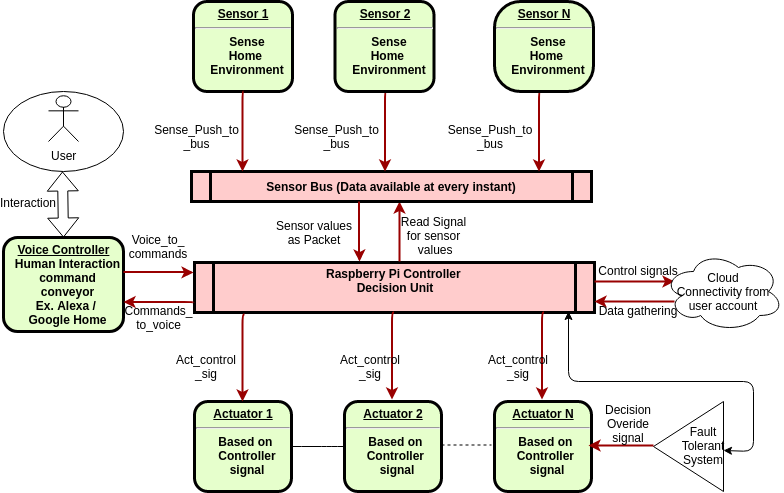
\includegraphics[width=\textwidth]{Home_Architecture.png}
    \caption{Home Architecture.}
  \end{minipage}
  \hfill
  \begin{minipage}[b]{0.4\textwidth}
    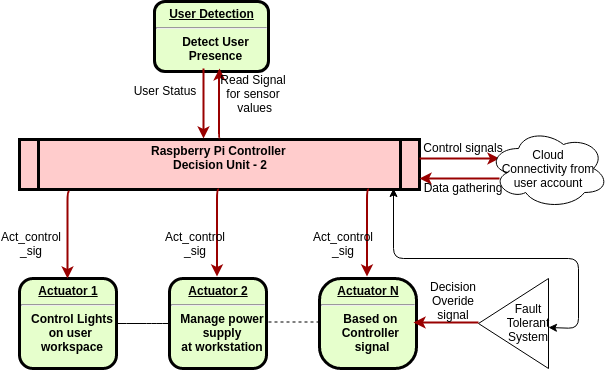
\includegraphics[width=\textwidth]{Office_Architecture-Page-1.png}
    \caption{Workplace Architecture.}
  \end{minipage}
\end{figure}

\begin{figure}
        \centering
        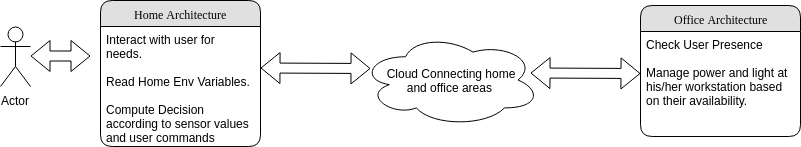
\includegraphics[width=1\textwidth]{System_Architecture.png}
        \caption{System overall Architecture}
        \label{fig:correctness}
    \end{figure}




\section{Requirements Specification}

For triggering actions at home and in the office, there has to be placed sensors and actuators.
The sensors at home and in the office are used to determine the presence of a user in each system. 
For the home systems a motion sensor, sound sensor and Google calendar API are used.
Based on the sensor output, the overall system can send message to the corresponding actuators and trigger actions. 

With the same sensor setup at the office, the corresponding actions are triggered. 
The sensors in each environment, also helps to evaluate, if the user is really present in the environment according to the information for the Google calendar. 
The actuators is used to turn  the power of specific device on or off based on the intelligent decision where the person is in a specific time period.

\section{Conclusions and Outlook}
An outline of a robust system is proposed to minimise the uncontrolled expenditure of energy and to provide a better lifestyle for the user. With this draft, the sensors that are a part of the smart network sense the parameters at home and workplace for the intelligent system to provide optimal living and working conditions that mainly emphasise on striking a balance between efficient usage of resources and comfortable lifestyle.

%
% ---- Bibliography ----
%
\bibliographystyle{splncs04}
\bibliography{mybib}

All links were last followed on April 17, 2019.

\end{document}
